\documentclass[10pt]{article}
\usepackage[left=2.54cm,top=2.54cm,right=2.54cm,bottom=2.54cm]{geometry}
\usepackage{fancyhdr}
\usepackage{afterpage}
\usepackage{setspace}
\usepackage{bibspacing}
\usepackage{booktabs} % To thicken table lines
\singlespacing

%%%% YOU CAN PUT YOUR OWN DEFINITIONS HERE
\newfont{\toto}{msbm10 at 12 pt}
\newfont{\ithd}{cmr9}
\newcommand{\equa}[1]{(\ref{eq:#1})}
\newcommand{\laeq}[1]{\label{eq:#1}}
\newcommand{\figu}[1]{\ref{fig:#1}}
\newcommand{\lafi}[1]{\label{fig:#1}}
\newcommand{\fmo}{\tilde{U}}
\newcommand{\fve}{\tilde{u}}
\newcommand{\Dt}{\Delta t}

\newcommand{\R}{\mathbb{R}}
\newcommand{\Z}{\mathbb{Z}}
\newcommand{\si}[1]{\rm\scriptscriptstyle{#1}}
\newcommand{\eqnref}[1]{(\ref{#1})} % To make parentheses automatically when referring to equations
\newcommand{\f}{\frac}
\newcommand{\lf}{\left}
\newcommand{\rg}{\right}
%\newcommand{\bm}[1]{\bm{#1}}
\renewcommand{\Im}{\operatorname{Im}}
\if@symbold\else\def\d{\,\mathrm{d}}\fi % the proper total derivative symbol

\newcommand{\ra}[1]{\renewcommand{\arraystretch}{#1}}
%%%% END OF YOUR DEFINITIONS

\pagestyle{fancyplain}
\renewcommand{\headrulewidth}{0pt}

\usepackage{amsmath,amsthm,amsfonts,amssymb}
%\usepackage[pdftex]{graphicx}
\usepackage[T1]{fontenc}
\usepackage{url}


\usepackage{xcolor}
\usepackage{amsmath}
%\usepackage[fleqn]{amsmath}
\usepackage{amsmath}
\usepackage{amstext}
\usepackage{graphicx}
\usepackage{epsfig}
\usepackage{enumitem}
\usepackage{listings}
%\usepackage{subfigure}
%\usepackage{algorithm}
%\usepackage{algorithmic} 
\usepackage{url}
%\usepackage{hyperref}
% Define custom color
\colorlet{mblue}{blue!40!black}
%\usepackage[bookmarks=true,bookmarksnumbered=true,colorlinks=true,linkcolor=mblue,citecolor=mblue,urlcolor=mblue]{hyperref}      
\usepackage{doi}
\usepackage{bm}
\usepackage{esdiff}
\usepackage{subfigure}
\usepackage{booktabs} 
\usepackage{multirow}


\title{
\bf Local Dynamic VGI Procedure
}
\author{
 Zelu Xu$^{1}$  \\\\
$^{1}$ Department of Aerospace Engineering, RPI, Troy, NY, USA\\
}
\date{}

\begin{document}
%%%% TITLE
\maketitle
\afterpage{\fancyhead{}}

%%%% ABSTRACT AND KEYWORDS
%\vskip0.5cm
\centerline{
\begin{minipage}[t]{150mm}
{\bf Abstract:}
%Finite element method with high-order methods analysis can provide accurate results for boundary layer problems. However, with only B-splines as basis functions, the computational cost is higher than conventional methods. It is also difficult to deal with triangle or hexagon meshes using B-splines. Thus it is attractive to combine B-splines, Bernstein and/or Lagrangian polynomials in different directions. To help with analysis choices, we studied a two dimensional heat transfer problem and compared several combinations of different basis functions.
\vskip0.2cm
{\it Keywords:} local dynamic.\\
\end{minipage}
}
\vskip0.5cm

%\setcounter{tocdepth}{3}
\tableofcontents

\newpage
%%%% MAIN PART
\section{Introduction}
%% will add more literature review
Germano~\textit{et al.} in ~\cite{germano1991dynamic}
\section{Governing Equations}
\label{solveUstrong}

We start by a linear convection-diffusion problem, first derive the Galerkin approximation. Start with the strong form PDE:

\begin{equation}
    \begin{aligned}
       \quad  a_{i} u_{,i} -(\kappa_{ij} u_{,i})_{,j} = f \\\label{eq:1}
    \end{aligned}
\end{equation}

a is the constant convection velocity and $\kappa$ is the kinematic viscosity. Using $\omega$ as the test function, neglect boundary conditions, we get 
\begin{equation}
    \begin{aligned}
       \quad \int_{\Omega}\omega( a_{i} u_{,i} -(\kappa_{ij} u_{,i})_{,j}) d\Omega =  \int_{\Omega}\omega f d\Omega\\\label{eq:2}
    \end{aligned}
\end{equation}

Approximate the weighting and solution space using finite element basis functions:
 
\begin{equation}
    \begin{aligned}
       \quad u^{h}  = \sum_{A = 1}^{n}u_{A}N_{A},   \\
       \quad \omega^{h}  = \sum_{A = 1}^{n}C_{A}N_{A} \\
    \end{aligned}\label{eq:3}
\end{equation}

We will end with 
\begin{equation}
    \begin{aligned}
       \quad (D_{AB} + K_{AB}) u^{h}_{B} = 0   \\\label{eq:4}
    \end{aligned}
\end{equation}

And
\begin{equation}
    \begin{aligned}
       \quad D_{AB}  &= \int_{\Omega}(N_{A,i}a_{i}N_{B})d\Omega , \\
        \quad K_{AB}  &=  \int_{\Omega}(N_{A,i}\kappa_{ij}N_{B,j})d\Omega \\
    \end{aligned}\label{eq:5}
\end{equation}


\section{VMS and local VGI formulation}
\subsection{RBVMS}
\label{solvec1}
From VMS formulation, we assume a coarse scale u, and a fine scale $u^{\prime}$, and split the problem into these two scales:

\begin{subequations}\label{eq:11}
\begin{align} 
 a(w^{h},u^{h}) + a(w^{h},u^{\prime})  &= (w^{h},f)\label{eq:11a} \\
 a(w^{\prime},u^{h}) + a(w^{\prime},u^{\prime})  &= (w^{\prime},f)\label{eq:11b} 
\end{align}
\end{subequations}


Now we assume the fine scale $u^{\prime}$ is related to the residual of the coarse scale $u^{h}$ by 

\begin{equation}
    \begin{aligned}
       \quad u^{\prime} = -\tau R(u^{h}) = -\tau (\mathcal{L} u^{h} - f)\\\label{eq:12}
    \end{aligned}
\end{equation}

So equation for coarse scale $\eqref{eq:11a}$ now can be written as:

\begin{equation}
a(w^{h},u^{h}) + M_{rbvms}(w^{h},u^{h})  = (w^{h},f)\label{eq:13}
\end{equation}

In order to solve for the $M_{rbvms}$ model, we apply the VGI procedure, we assume for a coarse grid solution field $u^{H}$ and a fine grid solution field $u^{h}$, both satisfy the governing equation, and The equation for these two scales are:  
\begin{equation}
    \begin{aligned}
       \quad a(w^{H},u^{H}) + M_{rbvms}(w^{H},u^{H})  &= (w^{H},f) \\
        \quad a(w^{h},u^{h}) + M_{rbvms}(w^{h},u^{h})  &= (w^{h},f) \\
    \end{aligned}\label{eq:14}
\end{equation}

Using $V \subset H^{1}(\Omega)$ denote the weighting function space, we use $V^{H} \subset V^{h} \subset V $, and thus $\omega^{H} = \omega^{h}$. Then the two equations become:

\begin{subequations}\label{eq:15}
\begin{align} 
 a(w^{H},u^{H}) + M_{rbvms}(w^{H},u^{H})  &= (w^{H},f) \label{eq:15a} \\
 \quad a(w^{H},u^{h}) + M_{rbvms}(w^{H},u^{h})  &= (w^{H},f)\label{eq:15b} 
\end{align}
\end{subequations}

Take $(15a)-(15b)$, we get our VGI rbvms model

\begin{equation}
M_{rbvms}(w^{H},u^{h}) - M_{rbvms}(w^{H},u^{H})  = a(w^{H},u^{H})-a(w^{H},u^{h})\label{eq:16} 
\end{equation}

\subsection{Local VGI}
In equation \ref{eq:16}, we have $u^h$ from the previous finite element solve, and we will reconstruct $u^H$ from local information of $u^h$. We locally coarsen the grid, thus the difference between $u^{H}$ and $u^{h}$ is local within one patch. For that patch (the element left and right to one node in $1D$ case), we will reach the following equation:

\begin{multline}
\sum_{e \subset \Omega^{p}}(-a_{i} \omega^{H}_{,i},  -\tau a_{j} u^{h}_{,j})_{e} - (-a_{i} \omega^{H}_{,i},  -\tau a_{j} u^{H}_{,j})_{\omega^{H}}  =\\
 (-\omega^{H}_{,i},  a_{j} u^{H}_{j})_{\omega^{H}}  + (\omega^{H}_{,i},  \kappa_{ij} u^{H}_{,j})_{\omega^{H}} -\sum_{e \subset \Omega^{p}}[(- \omega^{H}_{,i},  a_{j} u^{h}_{j})_{e}+(\omega^{H}_{,i},\kappa_{ij} u^{h}_{,j})_{e}]\label{eq:17} 
\end{multline}

We proposed a new procedure to determine $\tau$, this does not require a $\tau$ definition in priory, but rather we use an iteration method to dynamically compute $\tau$. \\

\begin{equation}
\tau = c_{1}h^{c_{2}}\label{eq:18} 
\end{equation}

We also choose a weighting function as:
\begin{equation}
    \begin{aligned}
       \quad \omega^{H}_{,i}  = \frac{1}{|\Omega^H|} \\
    \end{aligned}\label{eq:19}
\end{equation}

We end up with

\begin{multline}
c_{1}a^{T}a\bigg\{ \bigg (\sum_{e \subset \Omega^{p}} \int {h^{c2} u^{h}_{,i} } d\Omega\bigg )-\int {H^{c2} u^{H}_{,i}} d\Omega \bigg\}= \\ 
\quad  \int {- a_{i}u^{H}}d\Omega + \kappa_{ij} \int{u^{H}_{,j}}d\Omega - \bigg(\sum_{e \subset \Omega^{p}} \bigg\{a_{i}\int{- u^{h}}d\Omega + \kappa_{ij} \int{  u^{h}_{,j}}d\Omega \bigg\}\bigg)\label{eq:21} 
\end{multline}


Now the last thing is defining a reconstruction method for $u^{H}$ and $u^{H}_{,i}$, it can be a least square fit from all surrounding nodes. \\
\noindent In order to do that, we first need to solve the coefficient of the linear approximation, for each node, the matrix is:
\begin{equation}
\begin{bmatrix}

   1 & x_{1}  & y_{1}\\ 1 &  x_{2}  & y_{2} \\ 1 &  x_{3}  & y_{3}\\...
\end{bmatrix}
 *
 \begin{bmatrix}
 a_{0}  \\ a_{1} \\ a_{2}
 \end{bmatrix}
 =
  \begin{bmatrix}
 u(1)  \\  u(2) \\ u(3)  \\...
 \end{bmatrix}
\label{eq:22}
\end{equation}

\noindent when we solve for $a_{1}, a_{2}$, we have $u^{H}$ and $u^{H}_{i}$. \\
\subsection{Strongly imposed $u^{H}$ at Dirichlet boundaries}
It helps to reduce the overshoot at the boundary if we can strongly impose $u^{H}$ at Dirichlet boundaries. We will use the derivatives $a_1$ and $a_2$ from the least square fit, and determine $a_0$ from the upwinded boundary nodes around the node is interested. Figure \ref{SQmesh} shows the setup for c1 and strongly imposed $u^H$ for a square mesh. In order to determine which boundary node will be exactly fit, we take the node that forms the minimum angle with convection direction. In equation \ref{eq:SI}, $x_{I}$ is the node we are interested in compute $c_{1}$ value, $x_{Bi}$ is all the boundary node, we will pick the boundary node that minimize equation \ref{eq:SI}. In plot \ref{minDirection}, it will be node $X_{b3}$
\begin{equation}
    \begin{aligned}
       \quad min \frac{(x_{I}-x_{Bi})\cdot a}{|x_{I}-x_{Bi}|\cdot |a|}  \\
    \end{aligned}\label{eq:SI} 
\end{equation}

\begin{figure}[h!]
	\begin{center}
	\includegraphics[width=0.3\textwidth, clip]{./figure/xIxb.png}
	\end{center}
		\vspace{0mm}
    \caption{Find the boundary node that will be exactly satisfied in least square}
  	\label{minDirection}
\end{figure}

\subsection{Upwind $c_{1}$ at Dirichlet Outlet}
One additional thing we will do at Dirichlet outlet is upwind c1 at boundary node. This means c1 at Dirichlet outlet will take the information of its upwind node's value. It can be down through simply take the upwind value or a linear extrapolation. In this paper, we will directly use the upwind value in 1D case results. But the same idea can be extended to 2D and 3D.

\subsection{Time loop}
As described before, this solving process is iterative, for each solution filed, we will have to solve a instantaneous set of $g$, update the $c_{1}$ with a time step of $c_{1}$ and  $g$, and the result $u^{h}$ should be the solution field after this process converged. \\
\begin{equation}
    \begin{aligned}
       \quad c_{1}  = \frac{1}{1+dt}*c_{1}+\frac{dt}{1+dt}*g,   \\
    \end{aligned}\label{eq:23} 
\end{equation}

\section{Result and Discussion}

\subsection{1D results}
We did a 1D case with and without force. In figure \ref{feq0} and figure \ref{feq1}, the red circle is dynamic  $\tau$ result, the blue star is static $\tau$ result, and black line is Galerkin without stabilization. Top left figure is Pe = 125, top right is Pe = 12.5, bottom left is Pe = 1.25 and bottom right is Pe = 0.125.
\subsubsection{No force}
We first verify our approach using a $1D$ problem with analytical solution. It is a simple convection diffusion problem with both Dirichlet boundary condition $u^{h} = 0$ at $x=0$ and$u^{h} = 1$ at $x=1$, the convection speed is $-1$. We change diffusivity parameter $\kappa$ to get cell Peclet number range from 125, 12.5, 1.25 and 0.125. $c_2$ is 1 for the first two case, and $c_2$ is 2 for the last two.
The static $\tau$ is the following setup:
\begin{equation}
    \begin{aligned}
       \tau_1  &= h/(2*a) \\
       \tau_2  &= h^2/(4*\kappa) \\
       \tau &=\frac{1}{(\tau_1)^{-2}+9*(\tau_2)^{-2}}
    \end{aligned}\label{eq:2} 
\end{equation}
When we plot the Galerkin solution, static (Asymptotic) $\tau$ solution and dynamic procedure result. For the first three Peclet numbers, Galerkin solution shows strong oscillation while static $\tau$ and dynamic $\tau$ can stabilize the result. For the last case, the dynamic $\tau$ setup can converge back to the Galerkin solution. In figure \ref{feq0}, I plot every other data point except the last two for static and dynamic $\tau$ setup.  For the top two cases, there is almost no difference for the static $\tau$ and dynamic $\tau$ result. This indicate dynamic procedure can provide a good and accurate result for high Peclet number. Only the second last point is different for Pe = 1.25 case, and dynamic $\tau$ is actually better in prediction of the point's location. For the last case, we verified that with enough resolving of the boundary layer, Galerkin solution is stable and out dynamic procedure will give us back the Galerkin solution.
\begin{figure}[h!]
	\begin{center}
	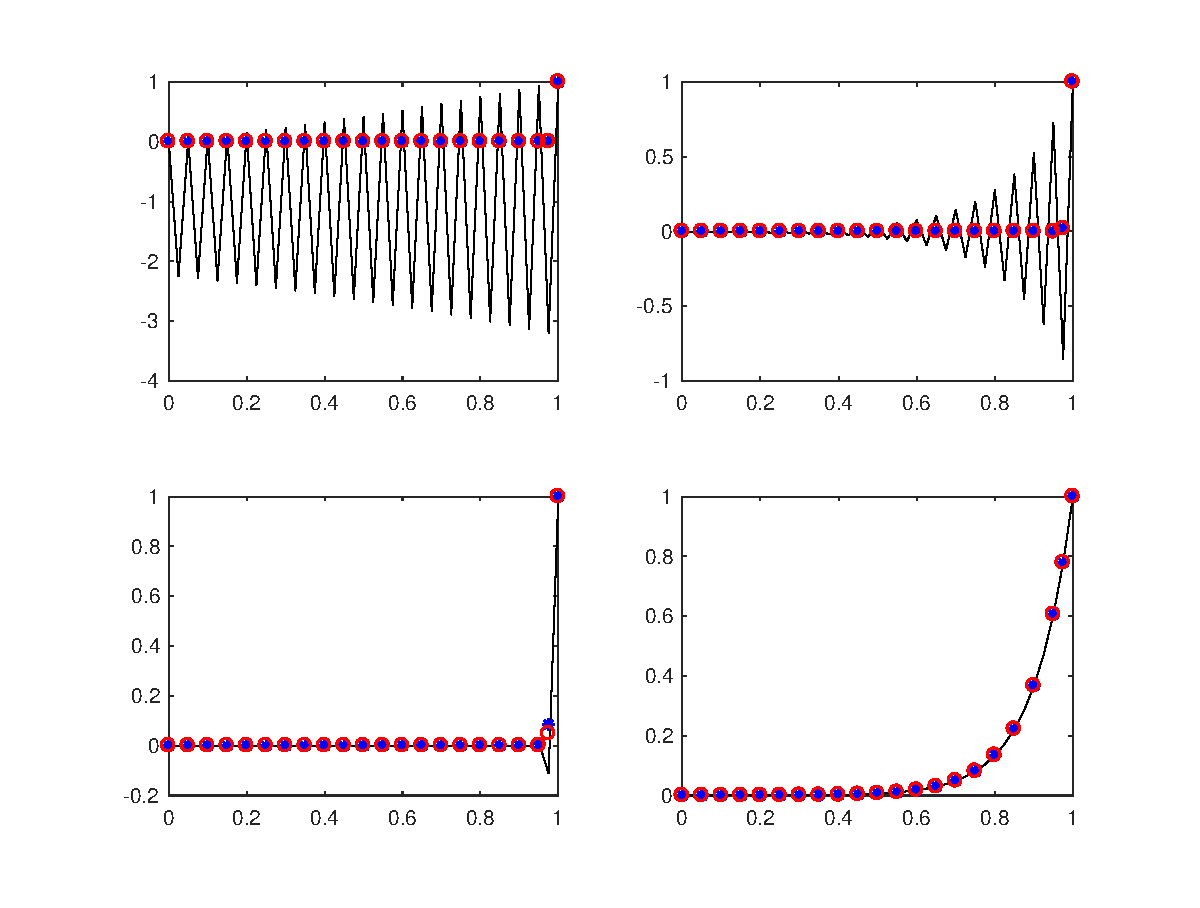
\includegraphics[width=1.0\textwidth, clip]{./figure/feq0.eps}
	\end{center}
		\vspace{0mm}
    \caption{1D Result with f=0 for Pe = 125, 12.5, 1.25,0.125 with Dynamic $\tau$ (red circle), Static $\tau$(blue star) and Galerkin(black line) setup}
  	\label{feq0}
\end{figure}
\subsubsection{With nonzero force}
This same comparison can be seen for the case with a force presented figure\ref{feq1}. This case we have a constant forcing term, and two Dirichlet condition both 0 at the two boundaries. Dynamic procedure also shows a good result when force is presented. It stabilize the result without too much diffusion and for high Peclet number, the result is very close to static asymptotic $\tau$. While for low Peclet number, it converge back to Galerkin solution
\begin{figure}[h!]
	\begin{center}
	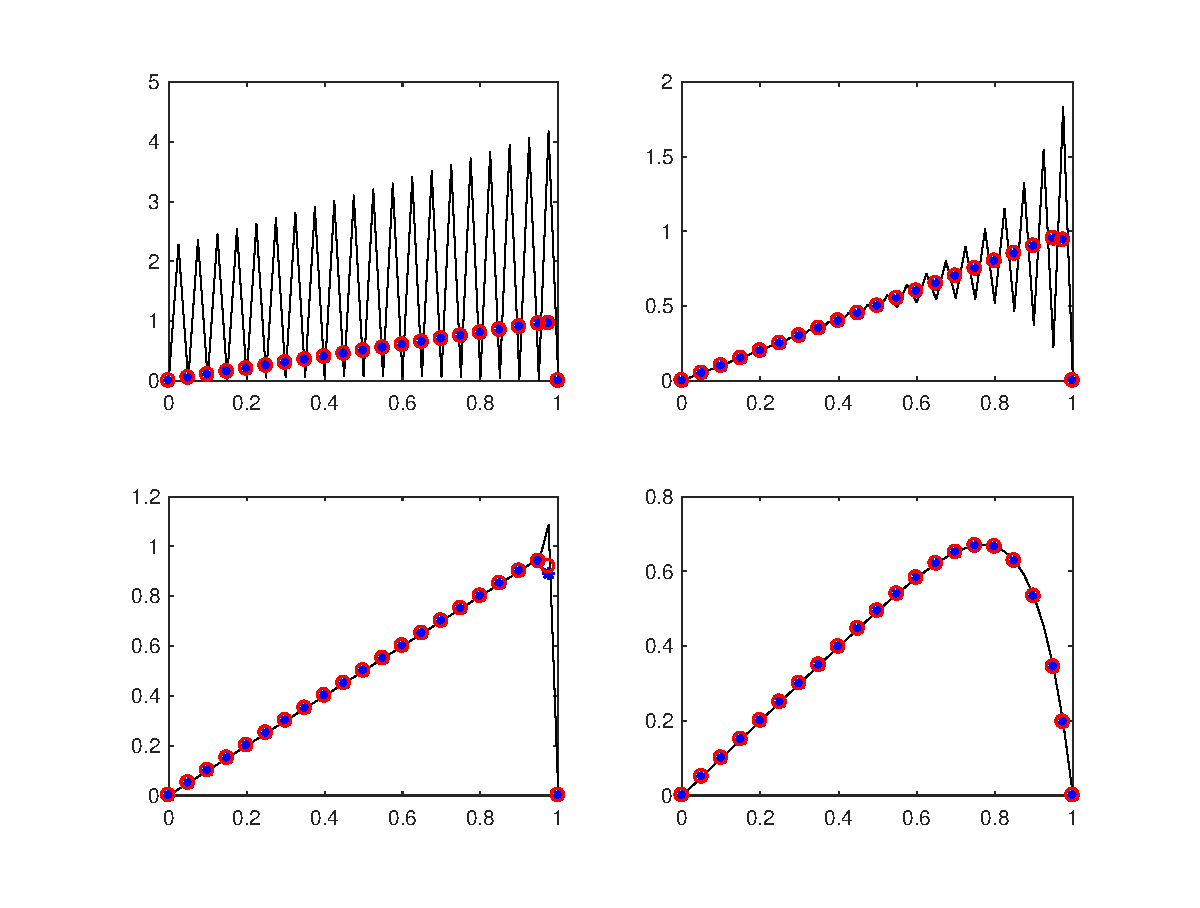
\includegraphics[width=1.0\textwidth, clip]{./figure/feq1.eps}
	\end{center}
		\vspace{0mm}
    \caption{1D Result with f=1 for Pe = 125, 12.5, 1.25,0.125 with Dynamic $\tau$, Static $\tau$ and Galerkin setup}
  	\label{feq1}
\end{figure}
\subsection{2D results}
The $2D$ problem I am evaluating has Dirichlet inlet boundary condition $u^{h} = 0$ at $x=0$ and $y=0$ The other two outlet boundary are 0 diffusive flux, the convection speed is $a = [1,1]$ and we change kappa to get a cell Peclet number 125, 12.5, 1.25 and 0.125.\\
The static asymptotic $\tau$ is calculated through a geometry $g_ij$ constant. The definition of $g_ij$ is related to the actual coordinate and Area of the element vertex.
\begin{equation}
    \begin{aligned}
       \tau_1  &= a*g_ij*a' \\
       \tau_2  &= 9(\kappa*g_ij)\cdot (\kappa*g_ij) \\
       \tau &=(\tau_1+\tau_2)^{-0.5}
    \end{aligned}\label{eq:2} 
\end{equation}
We show the result solved with both square mesh and a structured triangular mesh. For both of them, iteration start with the Galerkin solution. In figure \ref{SQ} and figure \ref{Tri}, the first row is for Pe=125, second row is Pe=12.5, third is Pe = 1.25 and last row is Pe = 0.125. For first and second row, $c_2$ = 1, while for last two rows, $c_2$ = 2. The first column is dynamic $\tau$ result, the second column is static $\tau$, the third one is Galerkin solution and the last column is a diagonal line plot at -45 degree of the first three column. For the last column, red circle is dynamic $\tau$ result, blue stat is static $\tau$, and black line is Galerkin solution. I plot every other data point for dynamic and static $\tau$ solution.
\subsubsection{Square Mesh}
We first solve the problem use a square mesh. The setup of problem and $c_1$ at boundaries can be seen as figure \ref{SQmesh}. For the two Dirichlet inlet, since the convection direction is at 45 degree angle, for each patch, we will exactly satisfy the least square fit at the -45 degree boundary node. For example, when we compute c1 for node 1, we will make sure the least square exactly fit the boundary value at node 2 as that is the most aligned direction. And for the actual boundary node2, $c_1$ is set to be 0. For the natural outlet boundaries, we will let $c_1$ calculated as a normal inertial node with less information(less node around a boundary). We also cut off at 0, which means if a calculated $c_1$ value is negative, we set it to be 0. We can do an absolute $c_1$ calculation, and in some case, it helps to get a more stable result, but in preventing of huge $c_1$ value, we decide to do the cutoff. And when we check, we did not get a lot of negative $c_1$s.
\begin{figure}[h!]
	\begin{center}
	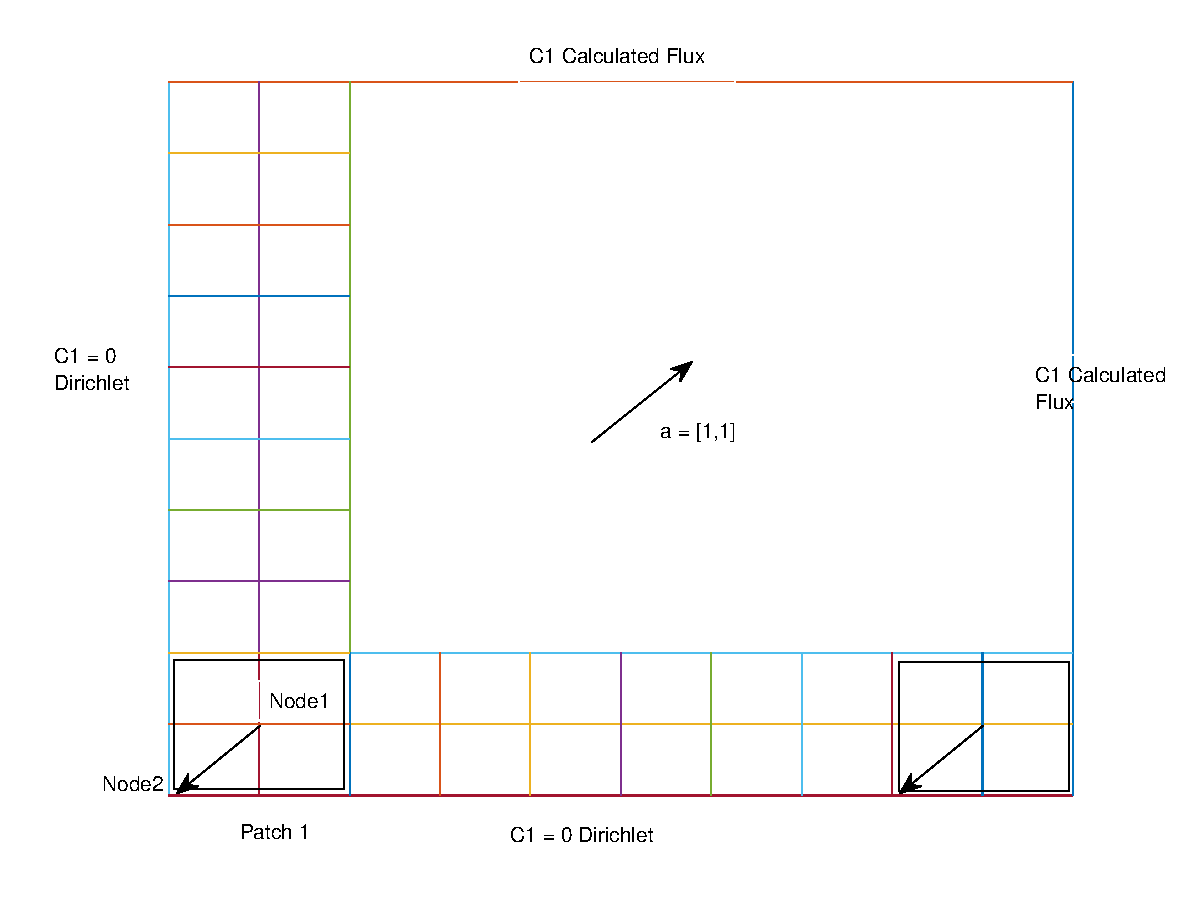
\includegraphics[width=0.65\textwidth, clip]{./figure/SQmeshGrid.eps}
	\end{center}
		\vspace{0mm}
    \caption{c1 setup near boundary for square mesh}
  	\label{SQmesh}
\end{figure}
In figure \ref{SQ}, for the first row with Pe = 125, our dynamic procedure can eliminate most of the oscillations. However, right after the drop, there is still a deep oscillation and a small one after this. The $u^h$ value is not different from the Galerkin solution, which means the local $c_1$ is very small and we do not have sufficient stabilization. The static case have a deeper oscillation, but with no secondary small oscillation. There is also a kink near the boundary for both static and dynamic $\tau$ case, but the kink is more obvious for the dynamic procedure.\\
For the case with Pe = 12.5, the Galerkin solution itself does not show a lot oscillation. But for both dynamic and static $\tau$, they still cannot fully resolve the kink near the boundary. This does not show up in the line plot as the line cut through -45 degree plane. \\
The last two rows show a good match with the Galerkin solution, thus the dynamic procedure will give back the Galerkin solution when the mesh can fully resolve the solution space.
\begin{figure}[h!]
	\begin{center}
	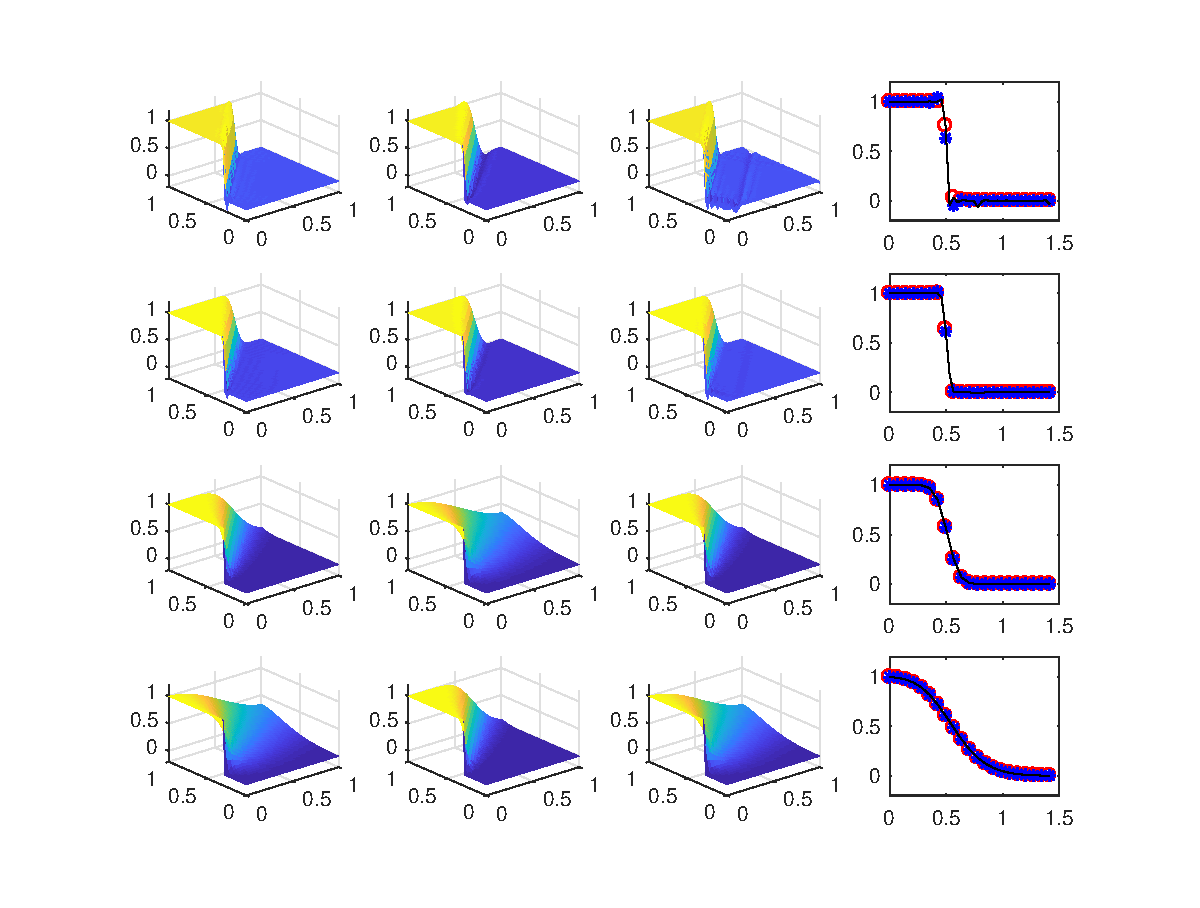
\includegraphics[width=1.0\textwidth, clip]{./figure/SQmesh.eps}
	\end{center}
		\vspace{0mm}
    \caption{Square Mesh Result for Pe = 125, 12.5, 1.25,0.125 with Dynamic $\tau$, Static $\tau$ and Galerkin setup}
  	\label{SQ}
\end{figure}
\subsubsection{Triangular Mesh}
We run the same case with a structured triangular mesh. The dynamic procedure solution is consistent with the square mesh result. For Pe = 125 case, the Galerkin solution shows more oscillations than the square mesh solution. The dynamic procedure result get rid off most the oscillations except the one right after the drop followed by another small one. While the static solution have only one oscillation but is wider and deeper. \\
The Pe = 12.5 dynamic case also have the kink near the boundary like the square mesh result, and the static $\tau$ solution resolve this kink better, but developed another dent after this kink.\\
For the resolved case Pe = 1.25 and Pe = 0.125, our dynamic procedure gives good consistency with Galerkin solution.\\
\begin{figure}[h!]
	\begin{center}
	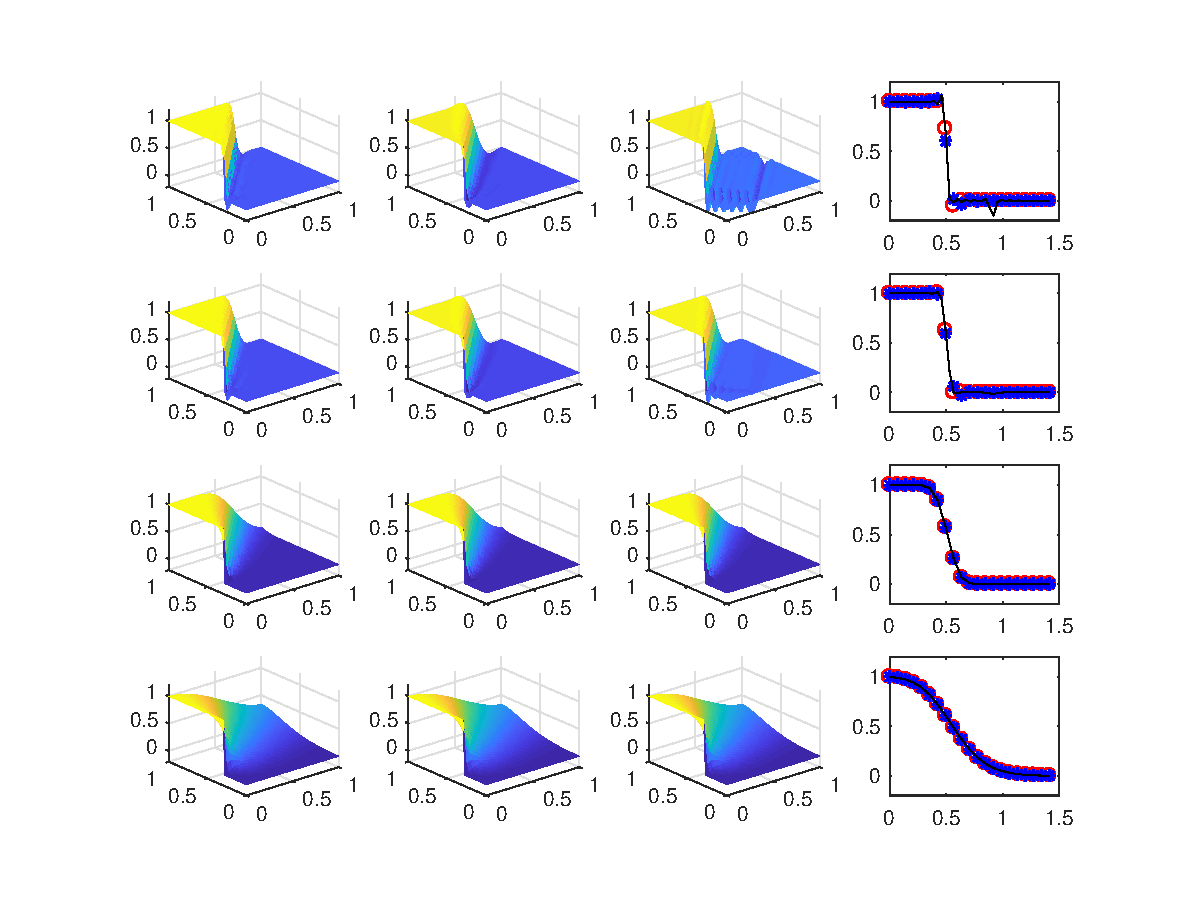
\includegraphics[width=1.0\textwidth, clip]{./figure/TRmesh.eps}
	\end{center}
		\vspace{0mm}
    \caption{Triangle Mesh Result for Pe = 125, 12.5, 1.25,0.125 with Dynamic $\tau$, Static $\tau$ and Galerkin setup}
  	\label{Tri}
\end{figure}


\subsection{Convergence Criteria and Error Estimation}
\label{error}
We stop the iteration if the iteration meets one of the two conditions. The first is norm of $u'^{h}$, which means if $\frac{norm(u'^{h}_{new}-u'^{h})}{norm(u'^{h}_{start})}$ is less than the tolerance set. The other one is if the coefficients of u is stable, which indicates if $\frac{||u^{h}_{iter+1}-u^{h}_{iter}||}{||u^{h}_{iter}||}$ is smaller than a set tolerance.  See figure \ref{Iteration} for the iteration convergence plot of the first criteria with Pe=125 case.See figure \ref{Iteration2} for the iteration convergence plot of the second criteria with Pe=125 case. Both of the value we watch for is decreasing fast during the first three iterations, and we stop the process if one of them is less than $10^{-3}$\\

\begin{figure}[h!]
	\begin{center}
	\includegraphics[width=0.75\textwidth, clip]{./figure/uprime.eps}
	\end{center}
		\vspace{0mm}
    \caption{$\frac{||u'^{h}_{new}-u'^{h})||}{||(u'^{h}_{start}||}$ with Iteration Numbers for Pe=125 2D case}
  	\label{Iteration}
\end{figure}

\begin{figure}[h!]
	\begin{center}
	\includegraphics[width=0.75\textwidth, clip]{./figure/unorm.eps}
	\end{center}
		\vspace{0mm}
    \caption{$\frac{||u^{h}_{iter+1}-u^{h}_{iter}||}{||u^{h}_{iter}||}$ with Iteration Numbers for Pe=125 2D case}
  	\label{Iteration2}
\end{figure}


%
%Now we need to introduce the stabilization term, because the first order Garlerkin approximation will oscillate for an under-resolved convection problem. We use the definition from VMS, we assume the stabilization term is related with the strong form residual of the governing equation, thus when residual approaches $0$, the additional stabilization term will also approach $0$. In mathematical, the stabilization term in linear elements will become:
%\begin{equation}
%    \begin{aligned}
%       \quad G_{stab} =   \int_{\Omega}a_{i}\omega_{,i} \tau R(u^{h}) d\Omega\\
%    \end{aligned}\label{eq:6}
%\end{equation}

%For a first order Garlerkin approximation, we only retain the first order derivative in the residual, thus 

%\begin{equation}
%    \begin{aligned}
%       \quad R(u^{h}) = a_{i} u^{h}_{,i}\\
%    \end{aligned}\label{eq:7}
%\end{equation}

%Thus:
%\begin{equation}
%    \begin{aligned}
%       \quad B_{AB}\cdot  u^{h}_{B} = F_{A}  \\
%    \end{aligned}\label{eq:8}
%\end{equation}

%with
%\begin{equation}
%    \begin{aligned}
%       \quad B_{AB}  &= \int_{\Omega}(N_{A,i}a_{i}N_{B})d\Omega +  \int_{\Omega}(N_{A,i}\kappa_{ij}N_{B,j})d\Omega +  \int_{\Omega} (a_{i} N_{A,i}) \tau (a_{j} N_{B,j})d\Omega, \\
%        \quad F_{A}  &=  \int_{\Omega}(N_{A}l)d\Omega \\
%    \end{aligned}\label{eq:9}
%\end{equation}

%After parametric coordinate transformation, the element stiffness matrix is 
%\begin{equation}
%    \begin{aligned}
%       \quad B_{ab}  &= \int_{0}^{1}(N_{a,i}a_{i}N_{b})\Box_{det}d\Box +  \int_{0}^{1}(N_{a,j}\kappa_{ij}N_{b,j})\Box_{det}d\Box +  \int_{0}^{1} (a_{i}N_{a,i})\tau (a_{j} N_{b,j})\Box_{det} d\Box \\
%    \end{aligned}\label{eq:10}
%\end{equation}

%We can then do the assembly of global stiffness matrix and force. \\

\section{Appendix}


%%%% BIBLIOGRAPHY
\bibspacing=\dimen 100
\bibliographystyle{unsrt}

\bibliography{master2}

\clearpage


\end{document}
